\documentclass[hyperref=colorlinks]{beamer}
\mode<presentation>
\usetheme{iclpt}
\setbeamertemplate{navigation symbols}{}
\setbeamertemplate{headline}{
\begin{beamercolorbox}[leftskip=.2cm,rightskip=.2cm,topskip=.2cm,ht=1.1cm,dp=0.1cm,wd=\textwidth]{institute in head/foot}
  
\includegraphics[height=1cm]{icl.pdf}
  \hfill
  
\includegraphics[height=1cm]{../Pics/CMS-Color.pdf}
\end{beamercolorbox}
}
\setbeamertemplate{footline}{
\begin{beamercolorbox}[ht=.55cm,dp=0.4cm,wd=\textwidth,leftskip=.3cm]{author in head/foot}%
  \begin{minipage}[c]{5cm}%
    \usebeamerfont{author in head/foot}
    \insertshortauthor 
    \insertshorttitle
    \end{minipage}\hfill%
  \insertframenumber{} / \pageref{lastframe}
  \hfill
  \begin{minipage}{6cm}
    \hfill
  \end{minipage}
\end{beamercolorbox}%
}

\usepackage{color}
\usepackage{tabularx,colortbl}
\usepackage{graphicx}
\usepackage{pdfpages}
\usepackage{feynmp}
\usepackage{multirow}
\DeclareGraphicsRule{*}{mps}{*}{}

\title{\vspace{-0.2cm} Higgs to Invisible MC Comparison}
%\subtitle{This result: HIG-15-012 \\ Contributing analyses: HIG-13-030, HIG-14-038, EXO-12-055}
%\author[P. Dunne]{\underline{P. Dunne} on behalf of the H$\rightarrow$invisible analysis group}
\titlegraphic{
  \vspace{-0.7cm}
  %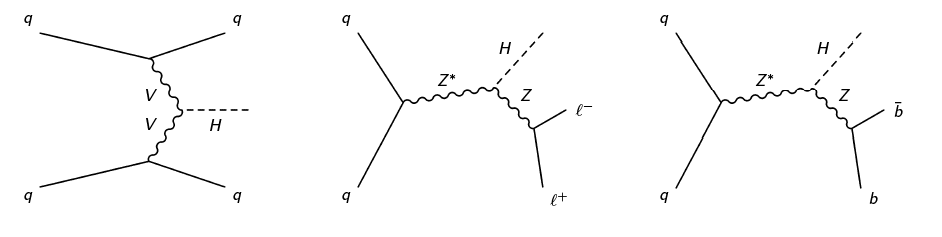
\includegraphics[width=\textwidth]{TalkPics/invcomb021213/feyndiags}
%% \begin{fmfgraph*}(100,70)
%%         \fmfleft{i1,i2}
%%         \fmfright{o1,o2,o3}
%%         \fmf{fermion}{i1,v1,o1}
%%         \fmf{fermion}{i2,v2,o3}
%%         \fmf{phantom,tension=4/5}{v1,v2}
%%         \fmffreeze
%%         \fmf{photon,label=$W,,Z$}{v1,v3}
%%         \fmf{photon,label=$W,,Z$}{v2,v3}
%%         \fmf{dashes}{v3,o2}
%%         \fmflabel{$q$}{i1}
%%         \fmflabel{$q$}{i2}
%%         \fmflabel{$q$}{o1}
%%         \fmflabel{$q$}{o3}
%%         \fmflabel{$H$}{o2}
%%       \end{fmfgraph*}
}
\date{}
\begin{document}
\begin{fmffile}{phenoplots141015feyndiags}

%TITLE PAGE
\section{Title}
\begin{frame}
  \titlepage
  
\end{frame}

%!!CLOSURE TEST STATEMENT PU jet ID
%OUTLINE
\begin{frame}
  \frametitle{Cut flow}
  \scriptsize
  \begin{block}{}
    \begin{itemize}
    \item Compare yields cut by cut
    \item Loosest selection easily available in CMS samples is: met significance$>3$, $\Delta\eta_{jj}>3.6$
    \item[-] all selection steps below have this requirement
    \item Add cuts one by one
    \end{itemize}
    \centering
  \end{block}
  \begin{block}{}
    \begin{tabular}{|l|c|c|}
      \hline
      Cut added & Powheg + CMS yield & Powheg + Delphes yield \\
      \hline
      $j_{1}p_{T}>50$, $j_{2}p_{T}>45$ & 1351 & 2655 \\
      min$\Delta\phi(j,met)>2.3$ & 649 & 1232 \\
      met$>90$ & 624 & 1221 \\
      \textcolor{red}{$M_{jj}>1200$} & 300 & 338 \\
      \textcolor{red}{met significance$>4$} & 273 & 286 \\
      \hline
    \end{tabular}
  \end{block}
\end{frame}

\begin{frame}
  \frametitle{Compare Distributions}
  \scriptsize
  \begin{block}{}
    \begin{itemize}
    \item Selection: met significance$>3$, $\Delta\eta_{jj}>3.6$
    \item These two variables were causing biggest cut flow difference before
    \item Met significance now seems fairly well modelled
    \end{itemize}
  \end{block}
  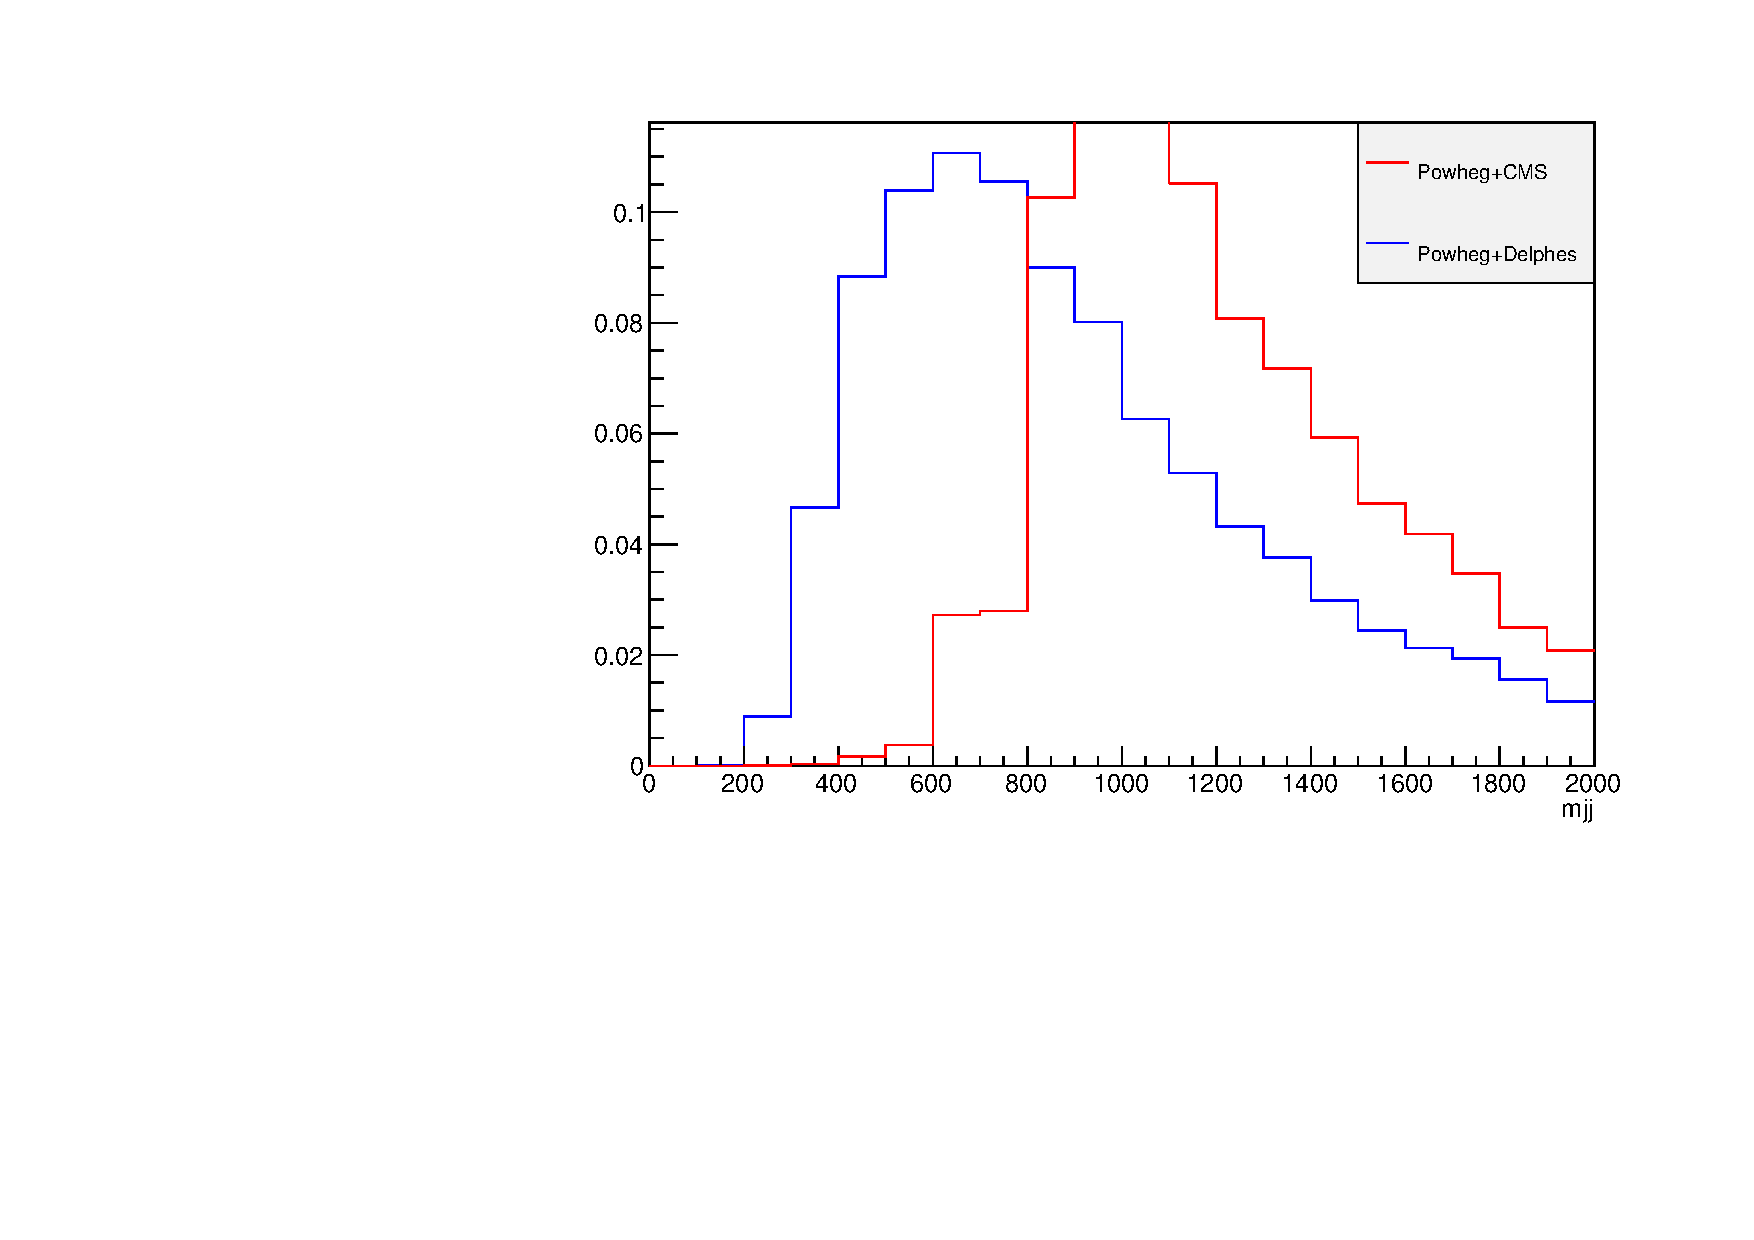
\includegraphics[width=.5\textwidth]{TalkPics/phenoplots201015/mjj_norm.pdf}
  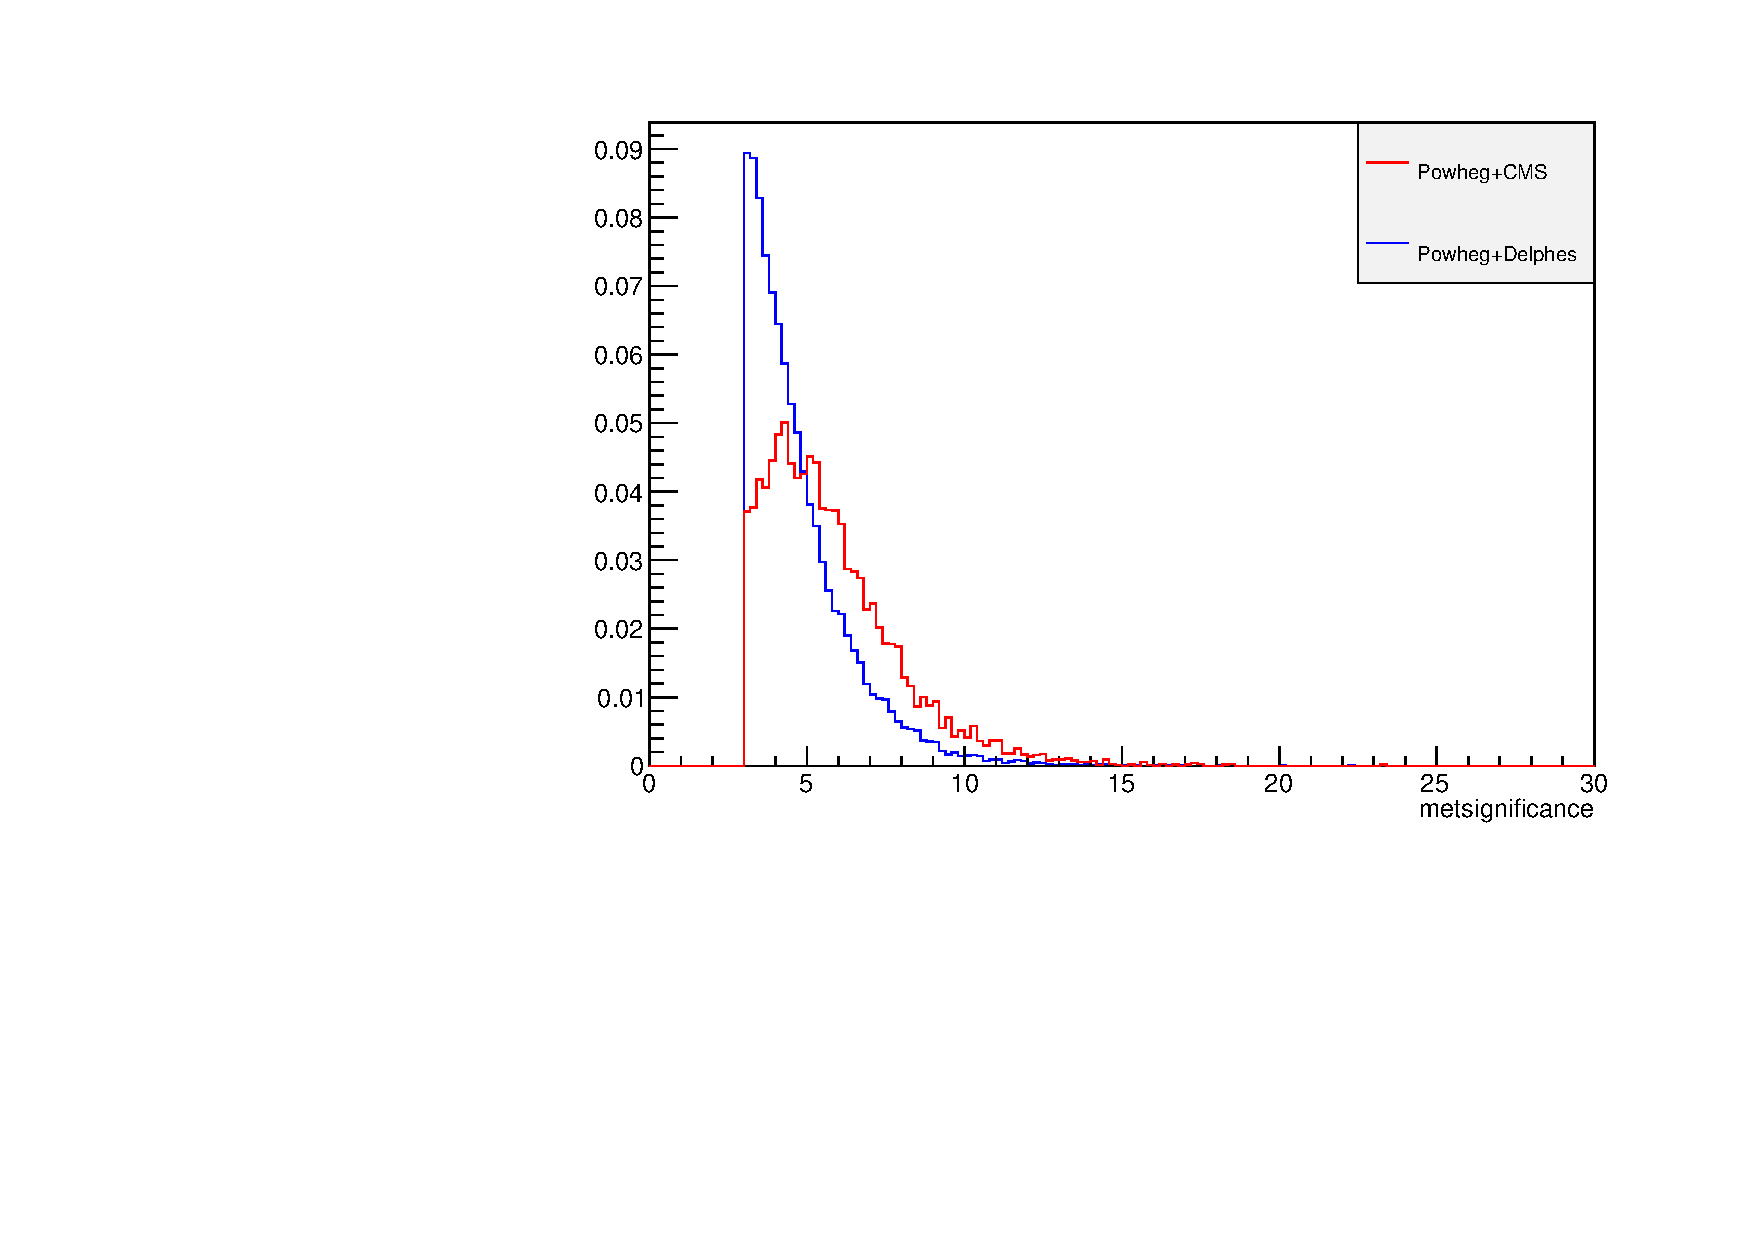
\includegraphics[width=.5\textwidth]{TalkPics/phenoplots201015/metsignificance_norm.pdf}
    
\end{frame}

\begin{frame}
  \frametitle{Compare Distributions}
  \scriptsize
  \begin{block}{}
    \begin{itemize}
    \item Selection: met significance$>3$, $\Delta\eta_{jj}>3.6$, $j_{1}p_{T}>50$, $j_{2}p_{T}>45$, min$\Delta\phi(j,met)>2.3$, met$>90$
    \item Jet pts fairly similar, a little harder in powheg
    \end{itemize}
  \end{block}
  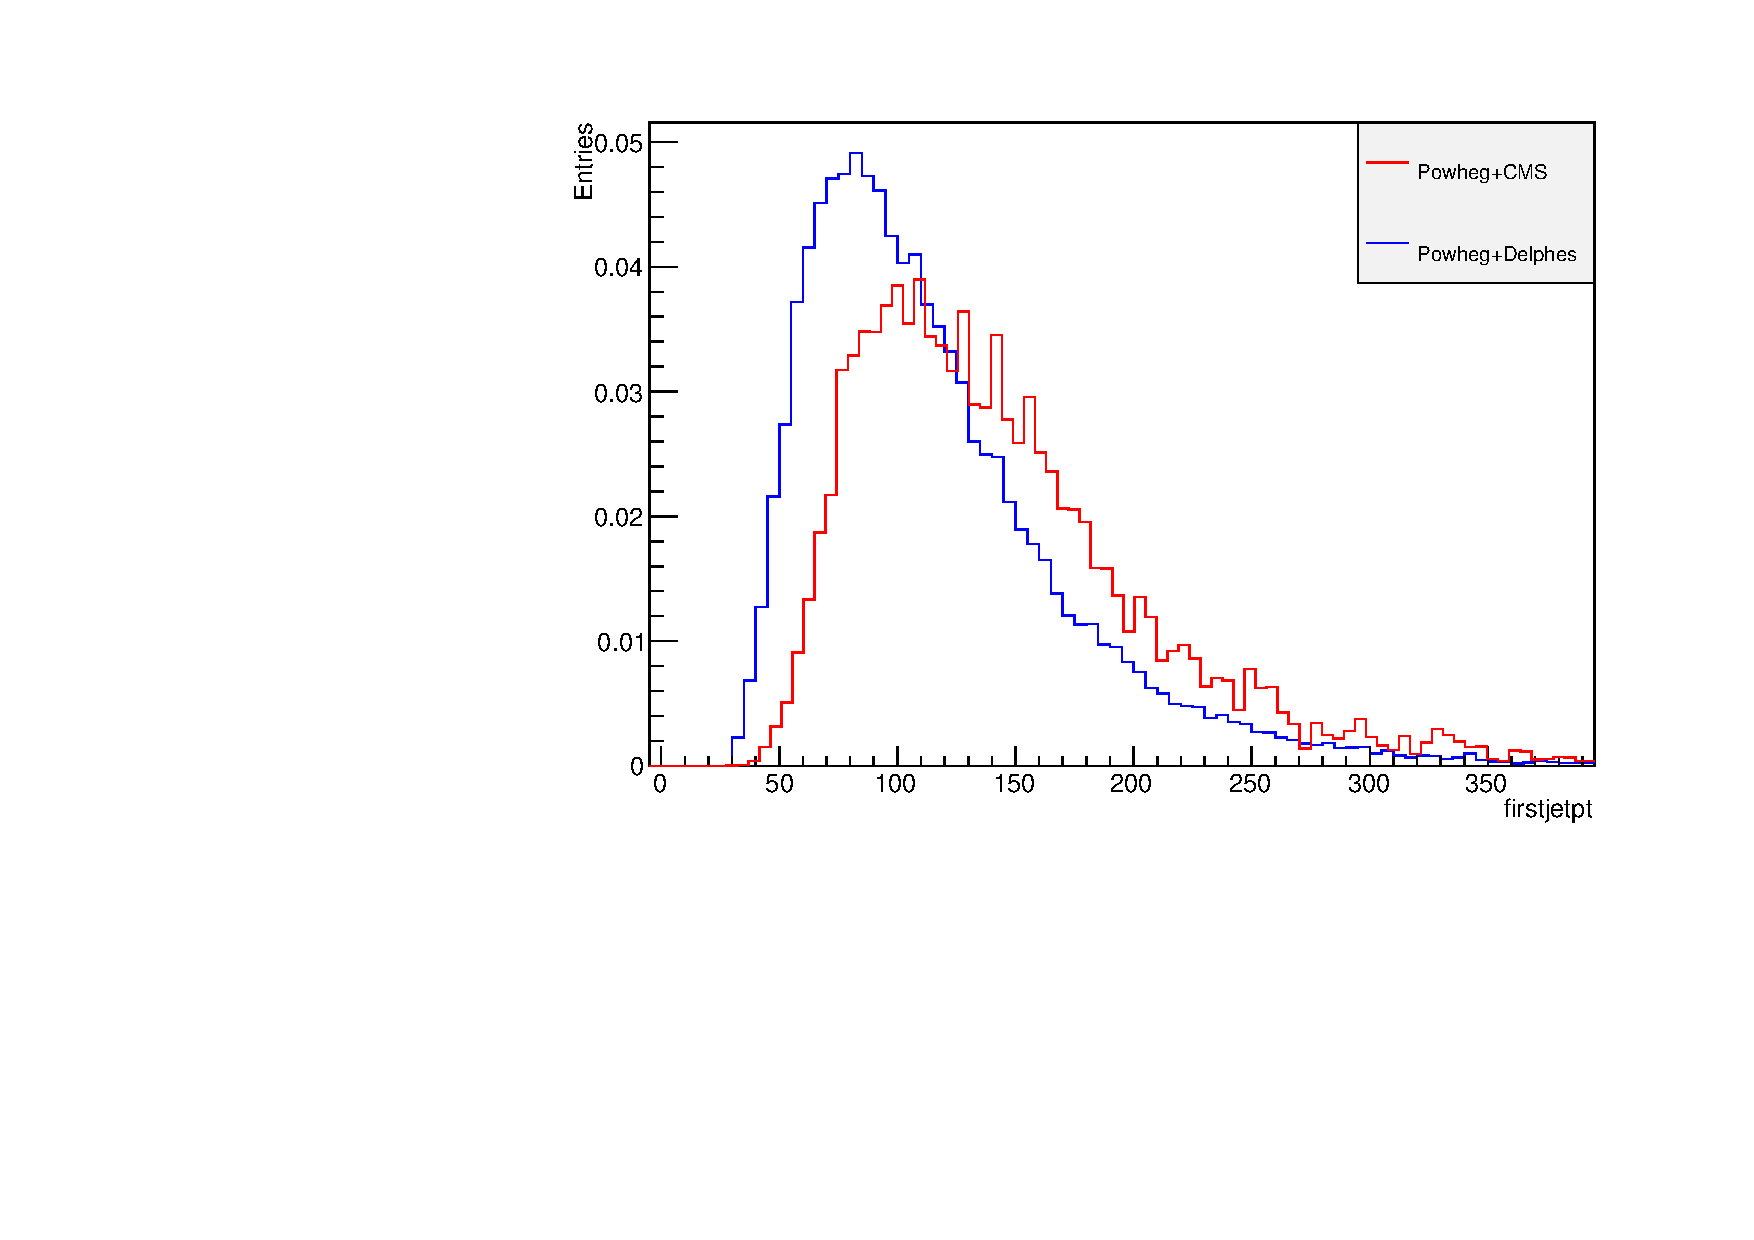
\includegraphics[width=.5\textwidth]{TalkPics/phenoplots201015/firstjetpt_norm.pdf}
  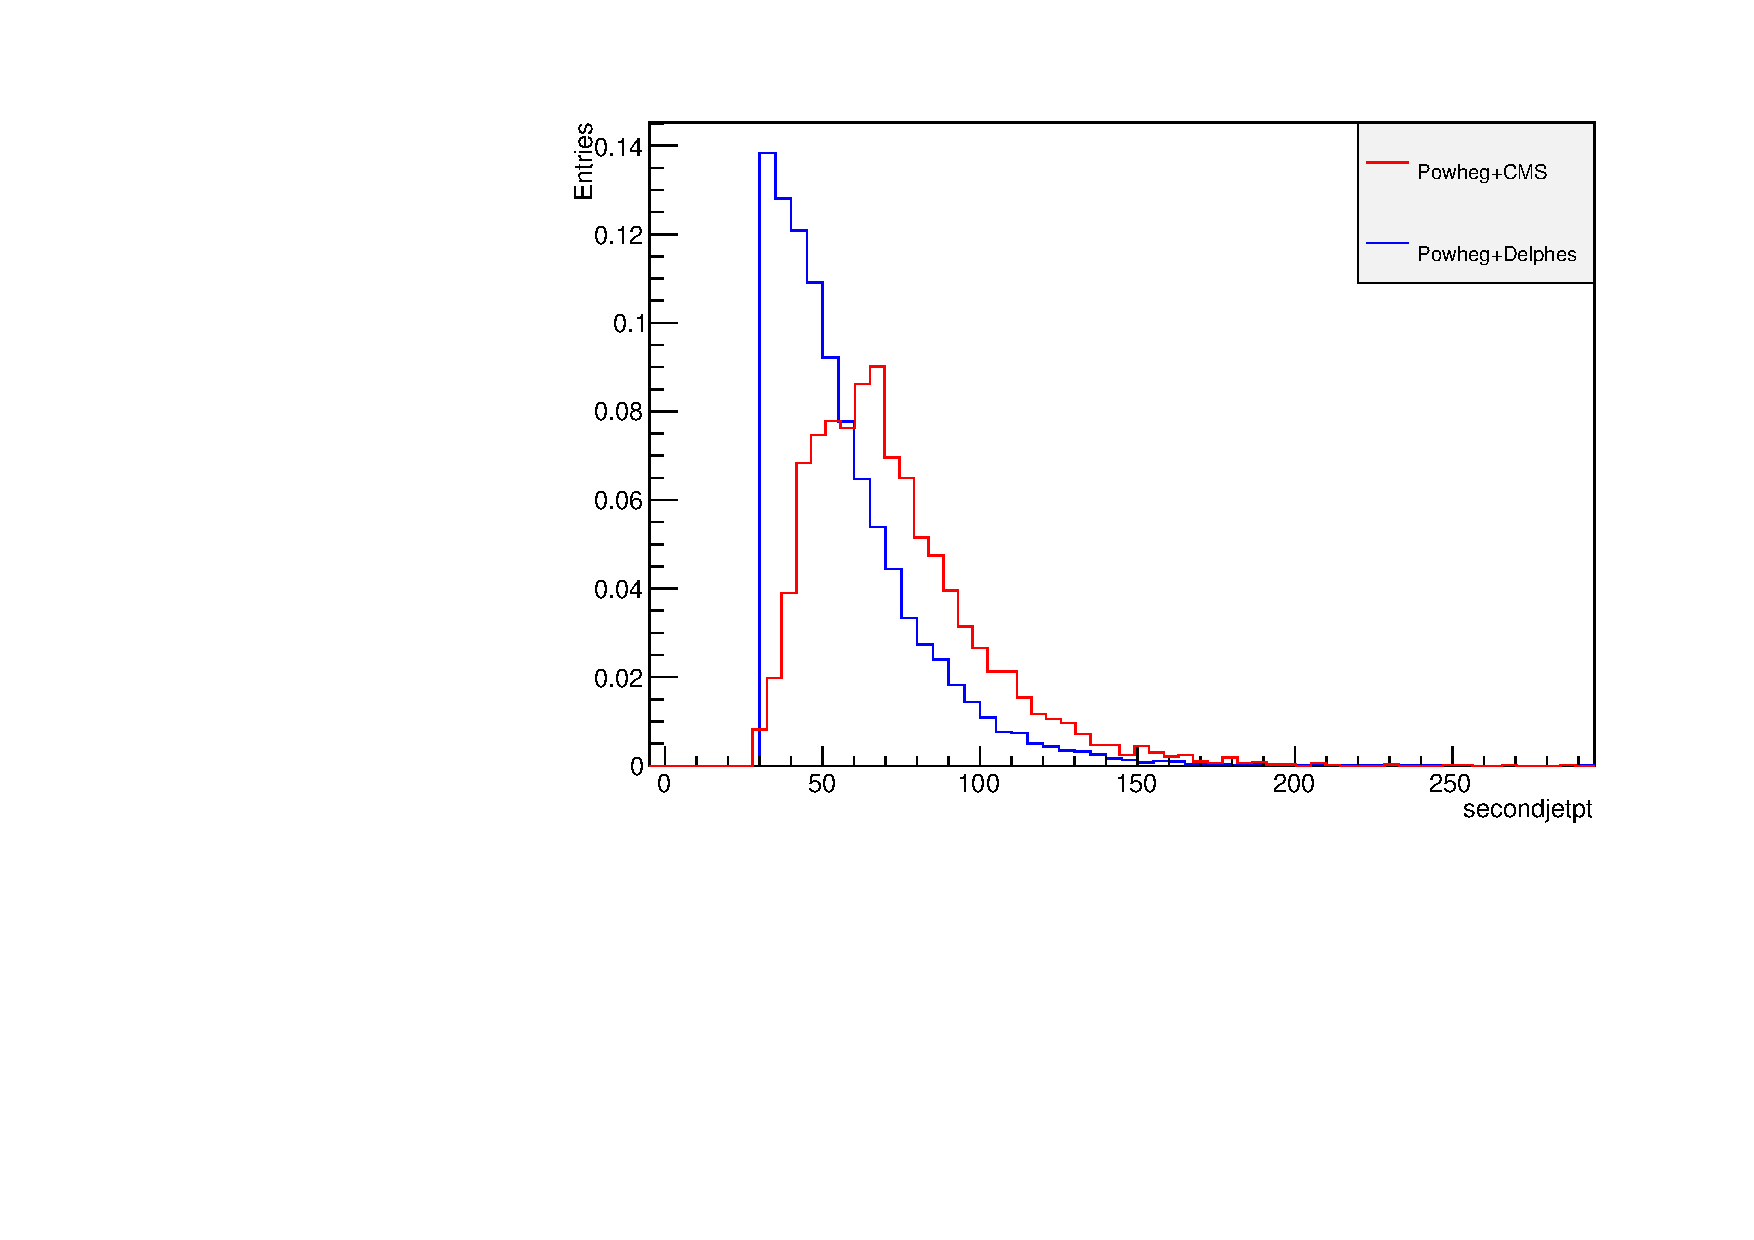
\includegraphics[width=.5\textwidth]{TalkPics/phenoplots201015/secondjetpt_norm.pdf}
    
\end{frame}

\begin{frame}
  \frametitle{Compare Distributions}
  \scriptsize
  \begin{block}{}
    \begin{itemize}
    \item Selection: met significance$>3$, $\Delta\eta_{jj}>3.6$, $j_{1}p_{T}>50$, $j_{2}p_{T}>45$, min$\Delta\phi(j,met)>2.3$, met$>90$
    \item Madgraph jets more central than powheg
    \end{itemize}
  \end{block}
  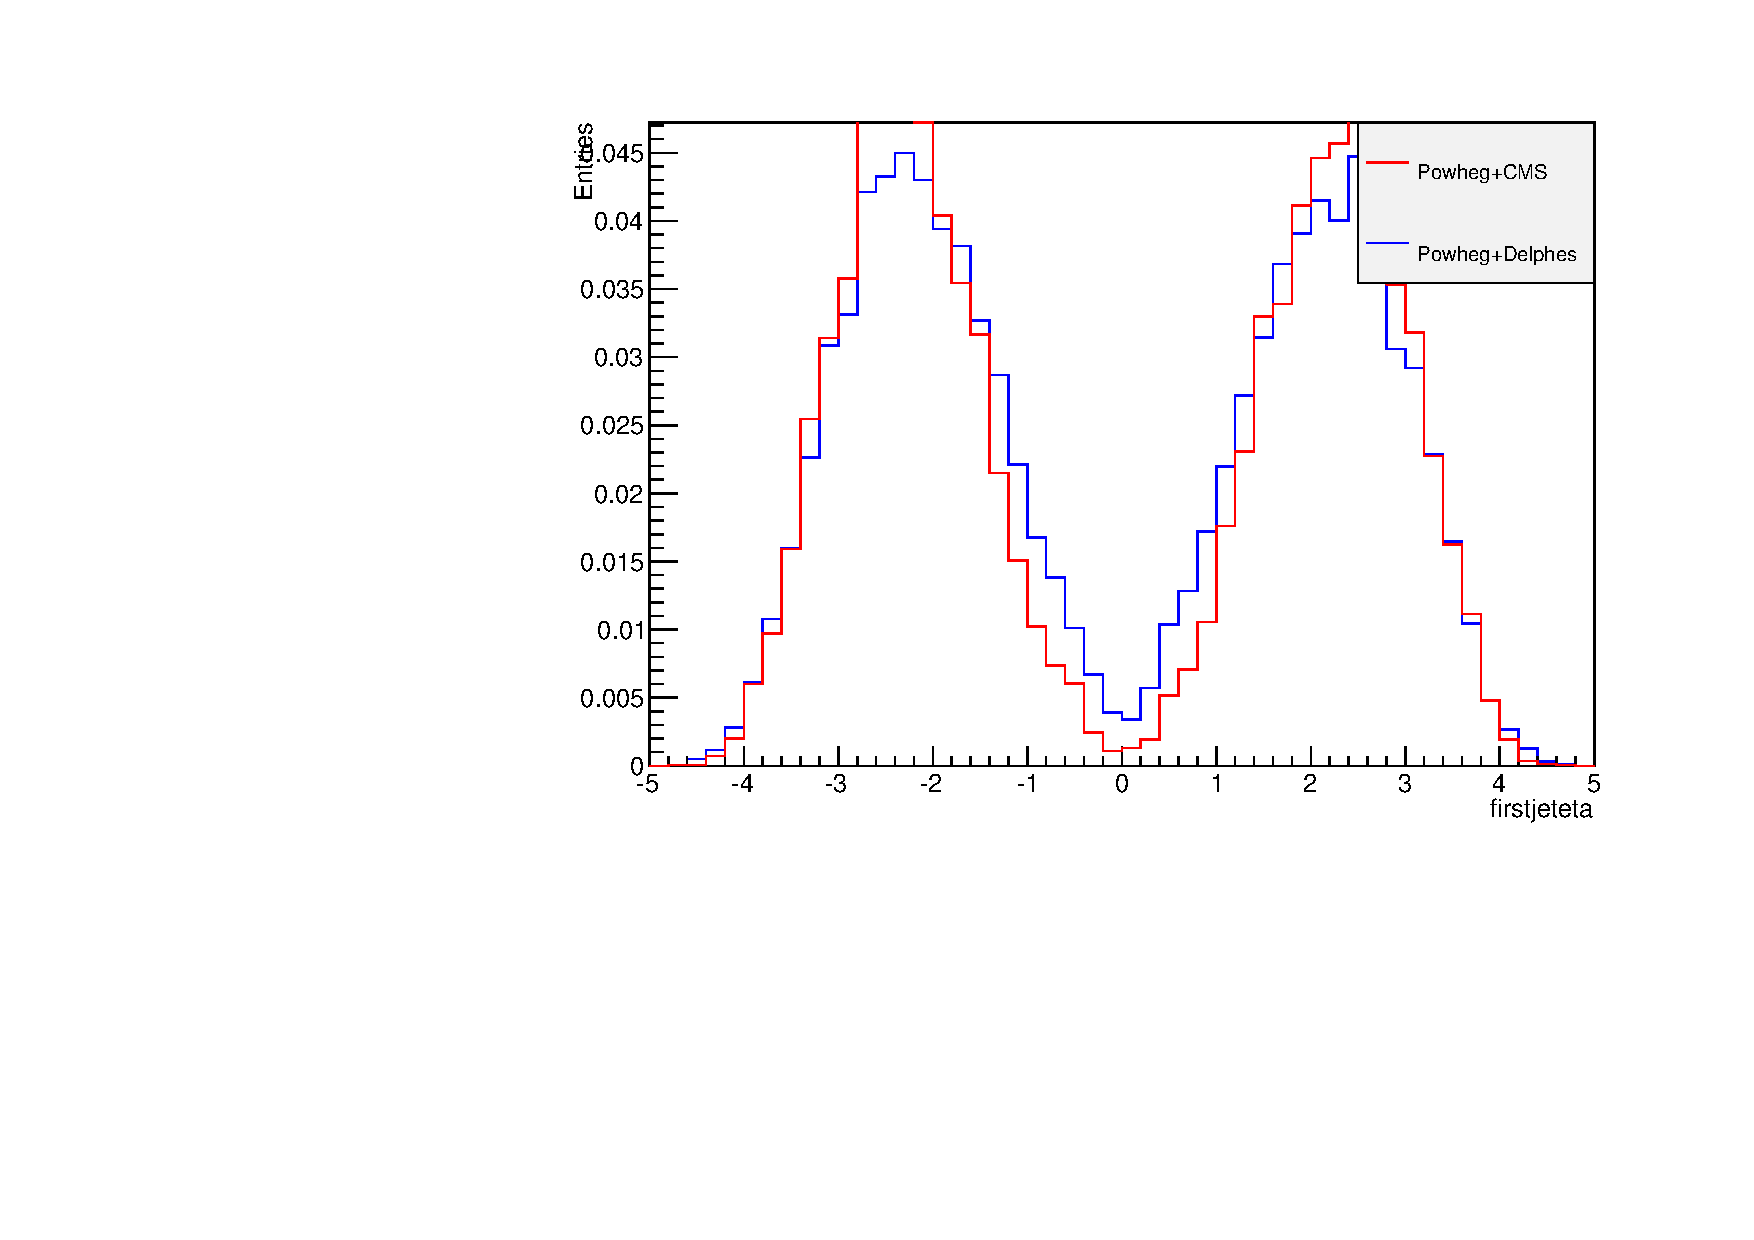
\includegraphics[width=.5\textwidth]{TalkPics/phenoplots201015/firstjeteta_norm.pdf}
  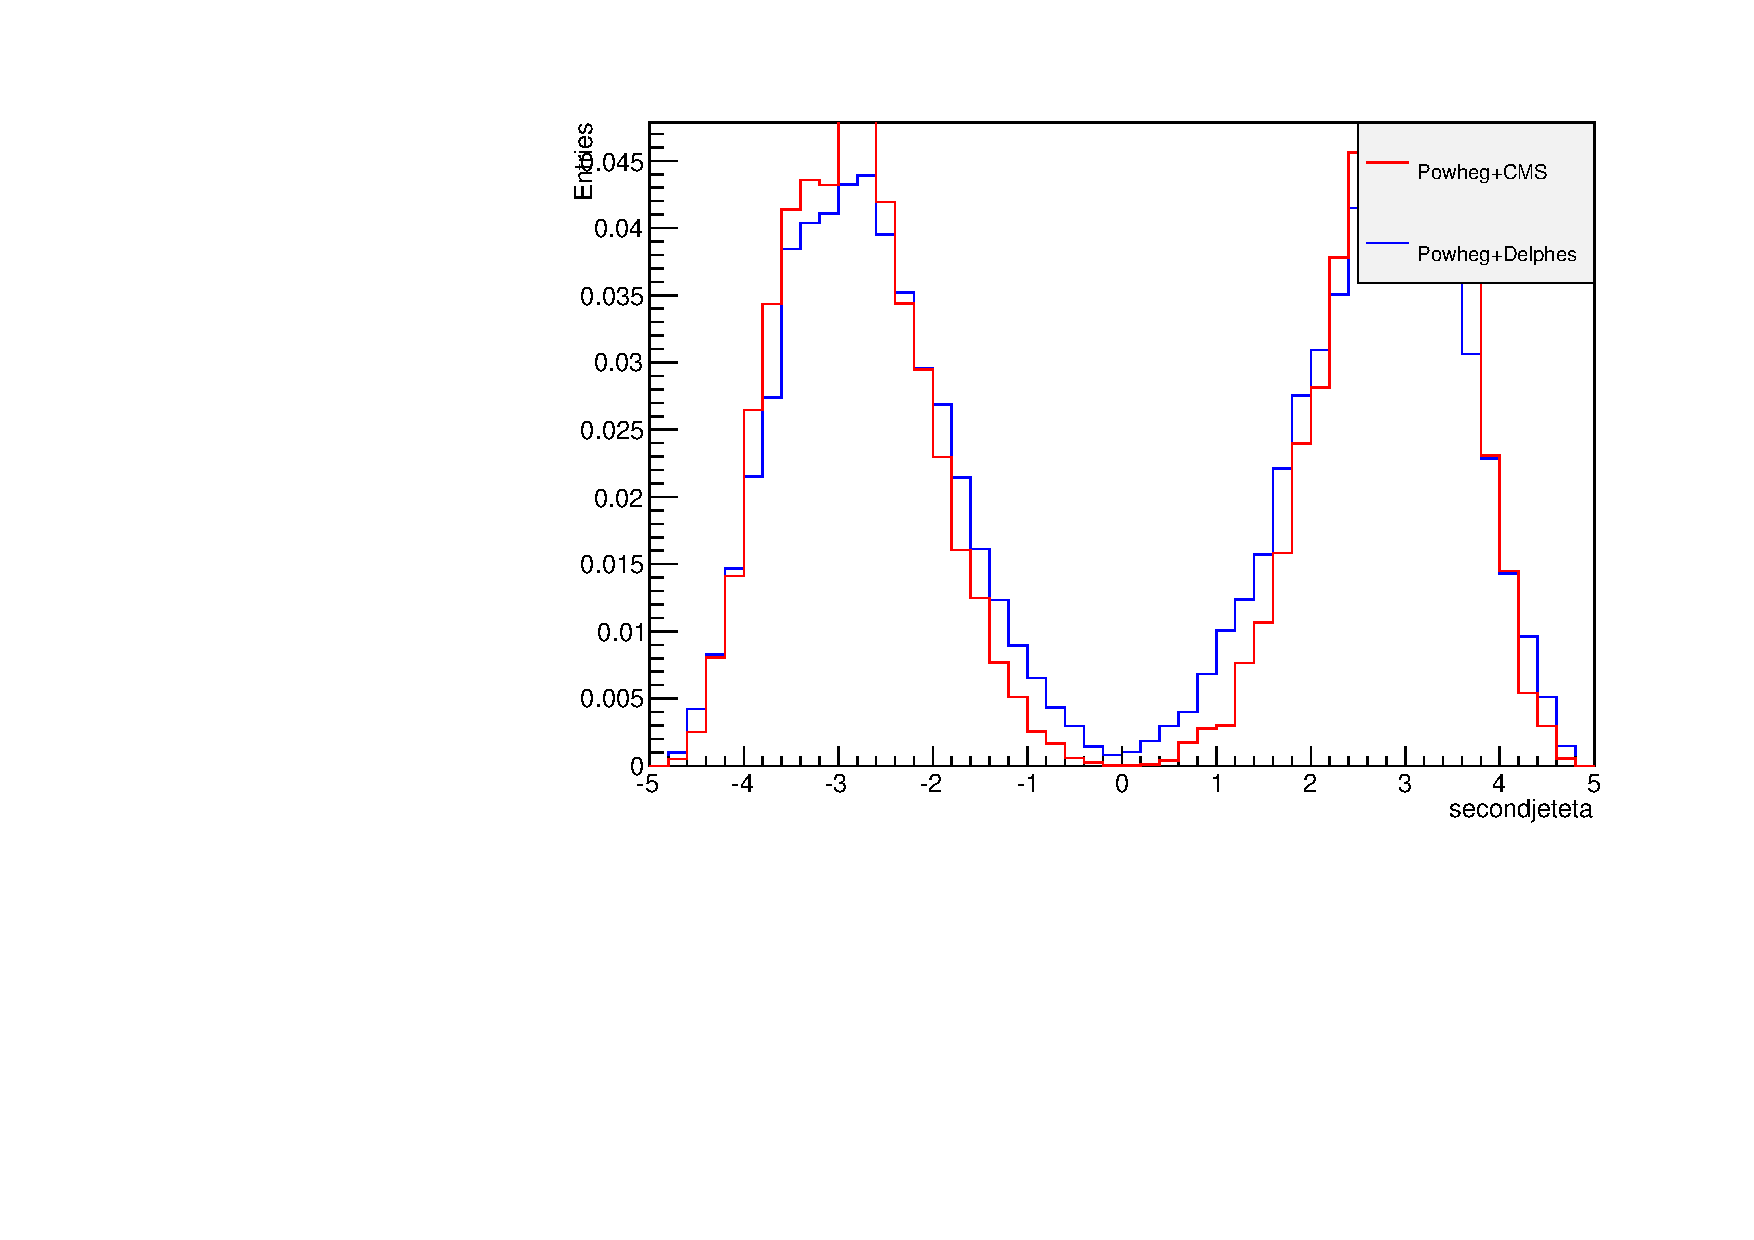
\includegraphics[width=.5\textwidth]{TalkPics/phenoplots201015/secondjeteta_norm.pdf}
    
\end{frame}

\begin{frame}
  \frametitle{Compare Distributions}
  \scriptsize
  \begin{block}{}
    \begin{itemize}
    \item Selection: met significance$>3$, $\Delta\eta_{jj}>3.6$, $j_{1}p_{T}>50$, $j_{2}p_{T}>45$, min$\Delta\phi(j,met)>2.3$, met$>90$
    \item Again see madgraph jets being more central
    \item Met similar between madgraph and powheg
    \end{itemize}
  \end{block}
  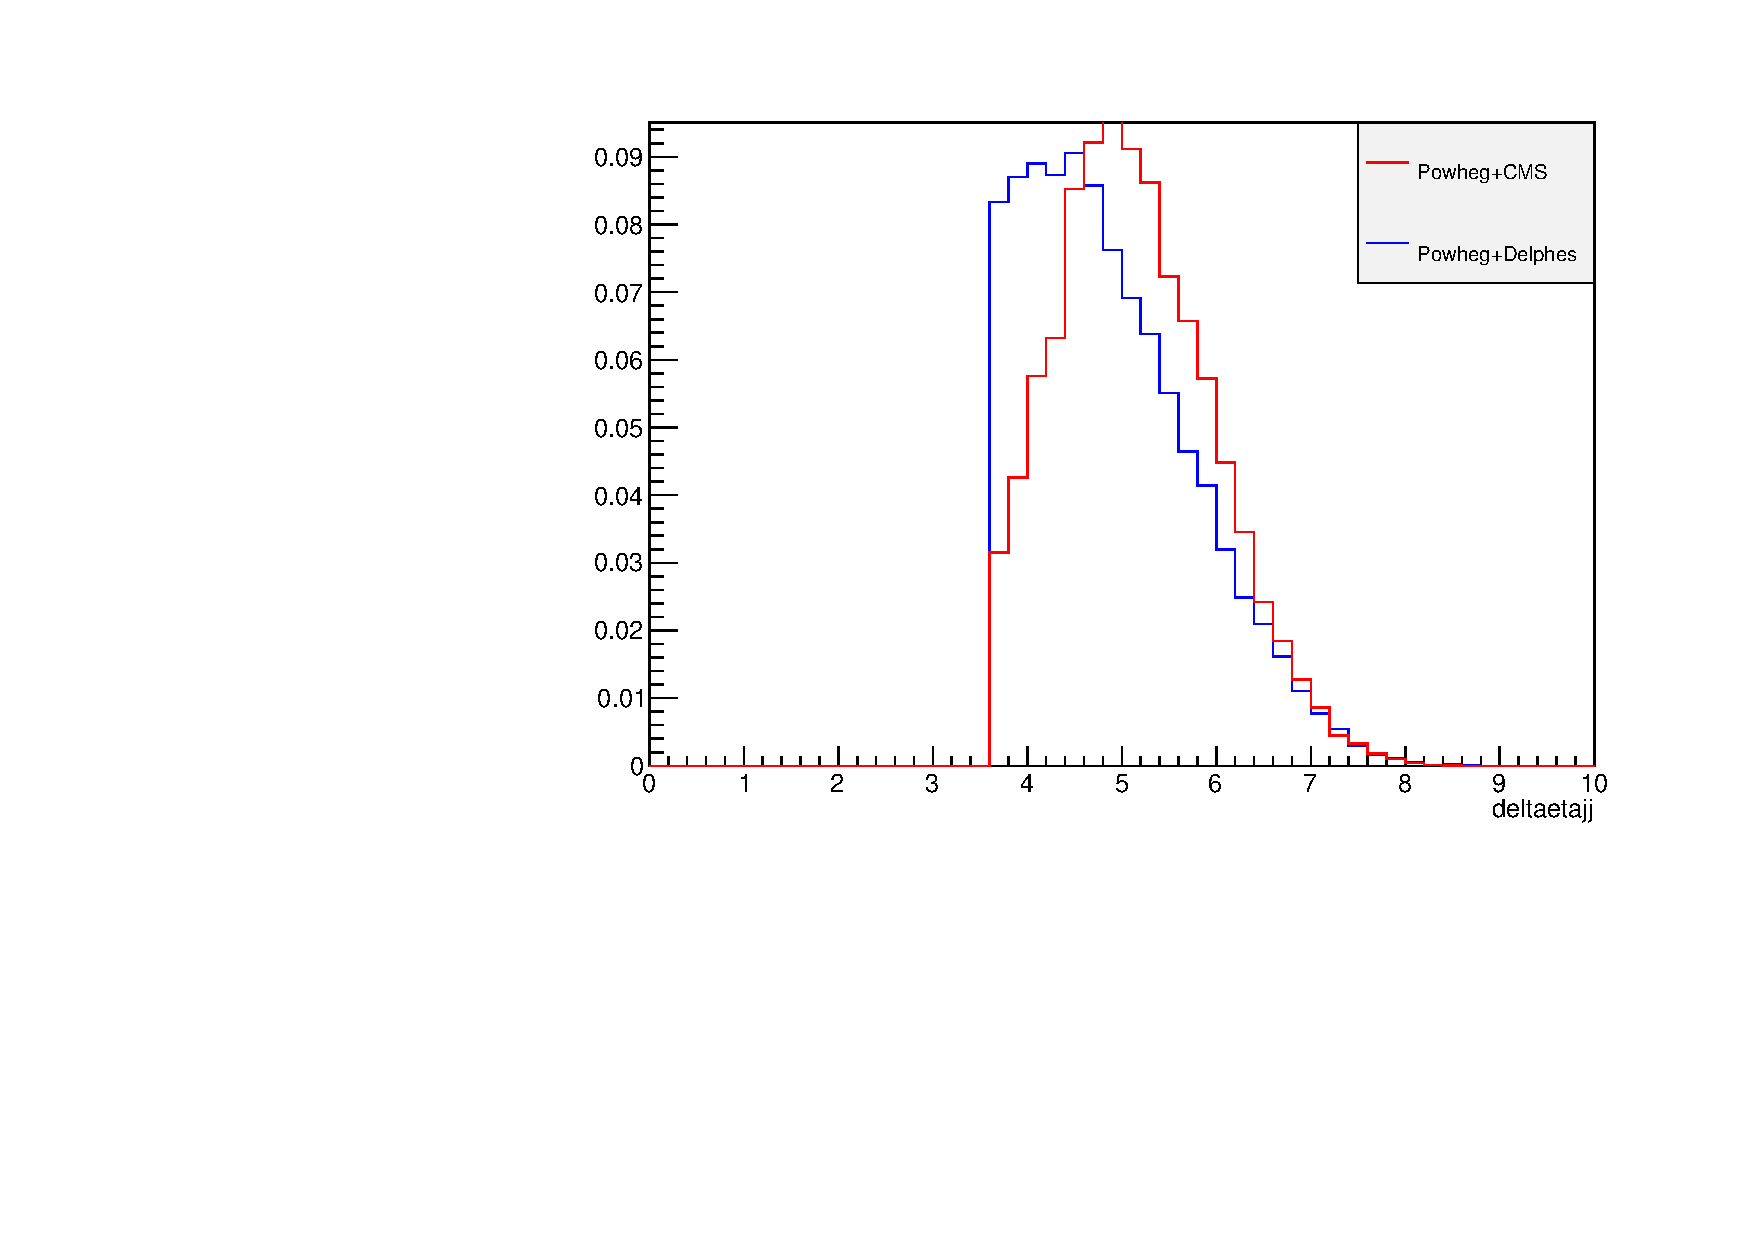
\includegraphics[width=.5\textwidth]{TalkPics/phenoplots201015/deltaetajj_norm.pdf}
  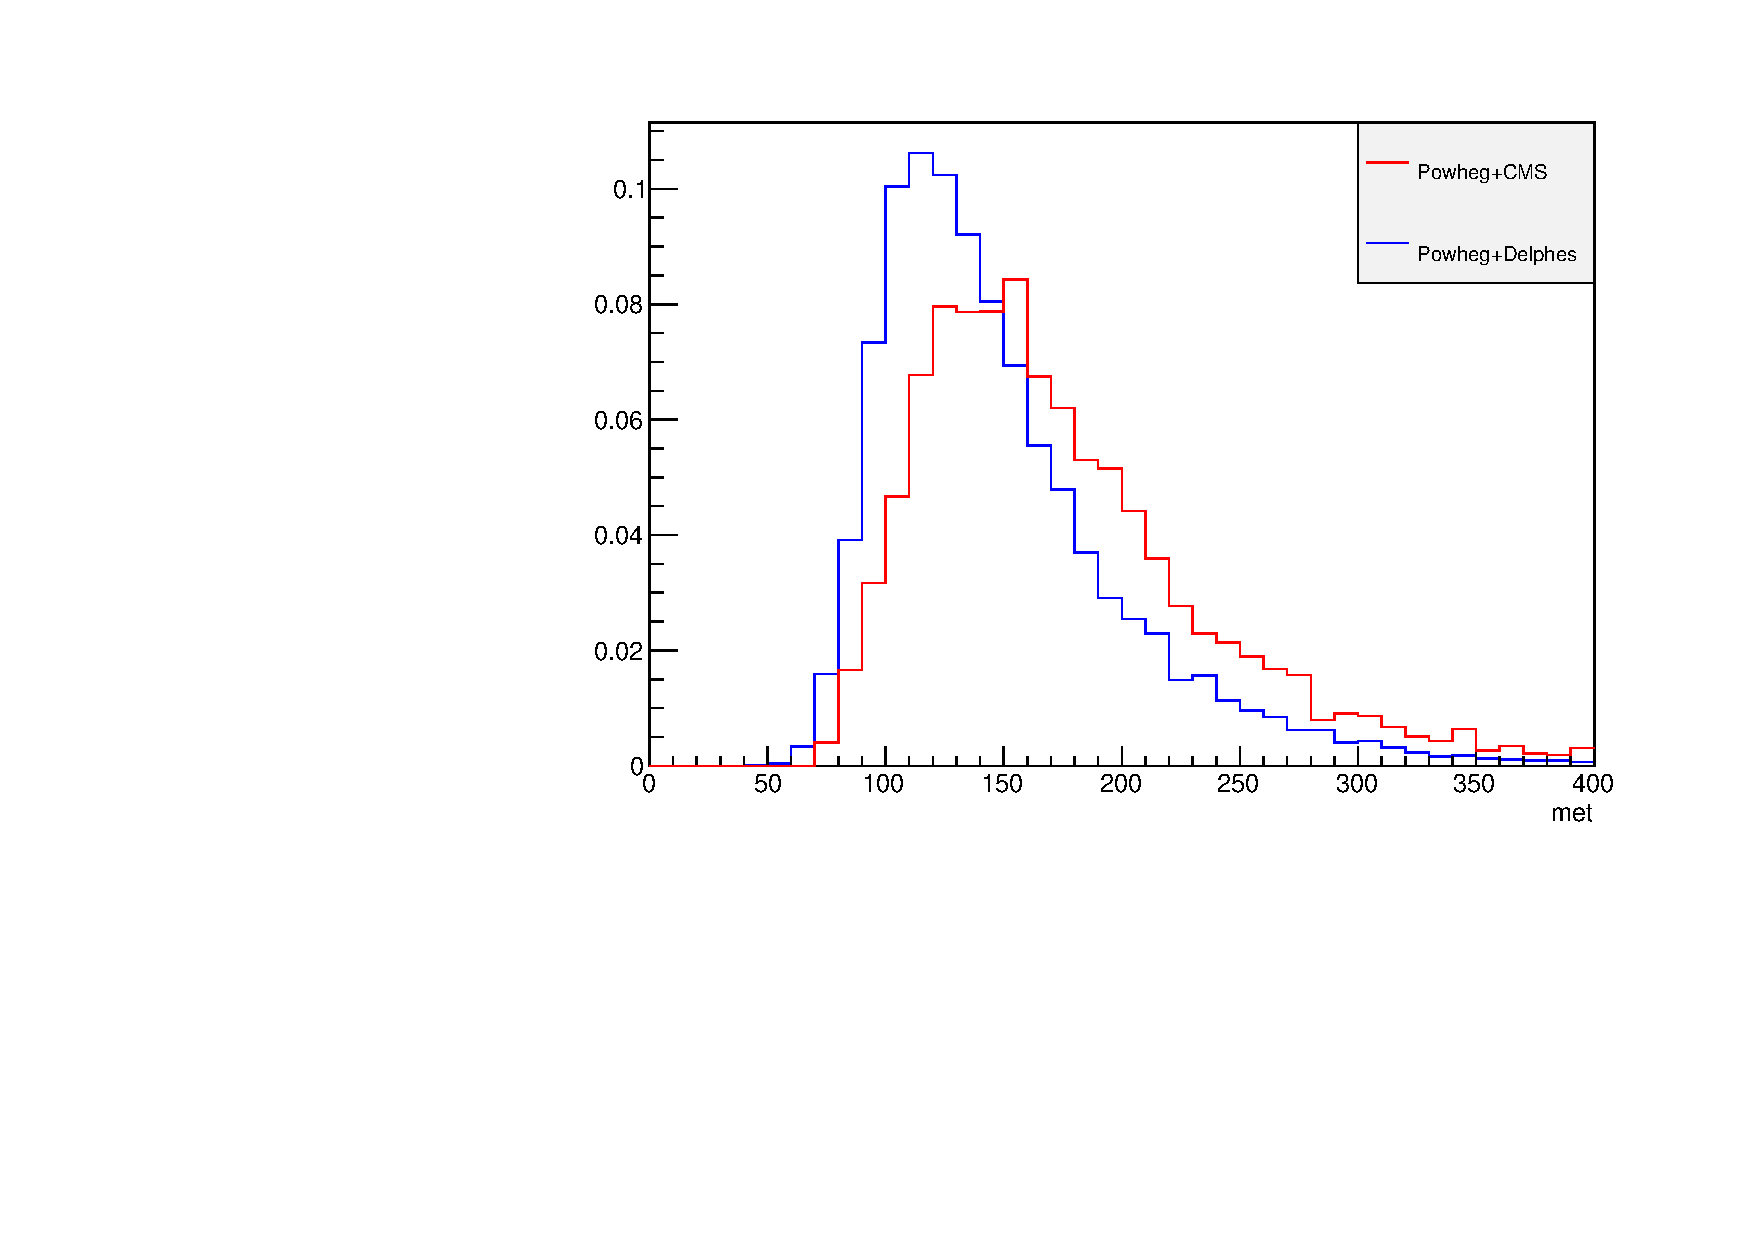
\includegraphics[width=.5\textwidth]{TalkPics/phenoplots201015/met_norm.pdf}
 
\end{frame}

\begin{frame}
  \frametitle{Compare Distributions}
  \scriptsize
  \begin{block}{}
    \begin{itemize}
    \item Selection: met significance$>3$, $\Delta\eta_{jj}>3.6$, $j_{1}p_{T}>50$, $j_{2}p_{T}>45$, min$\Delta\phi(j,met)>2.3$, met$>90$
    \item Limited statistics in phi
    \end{itemize}
  \end{block}
  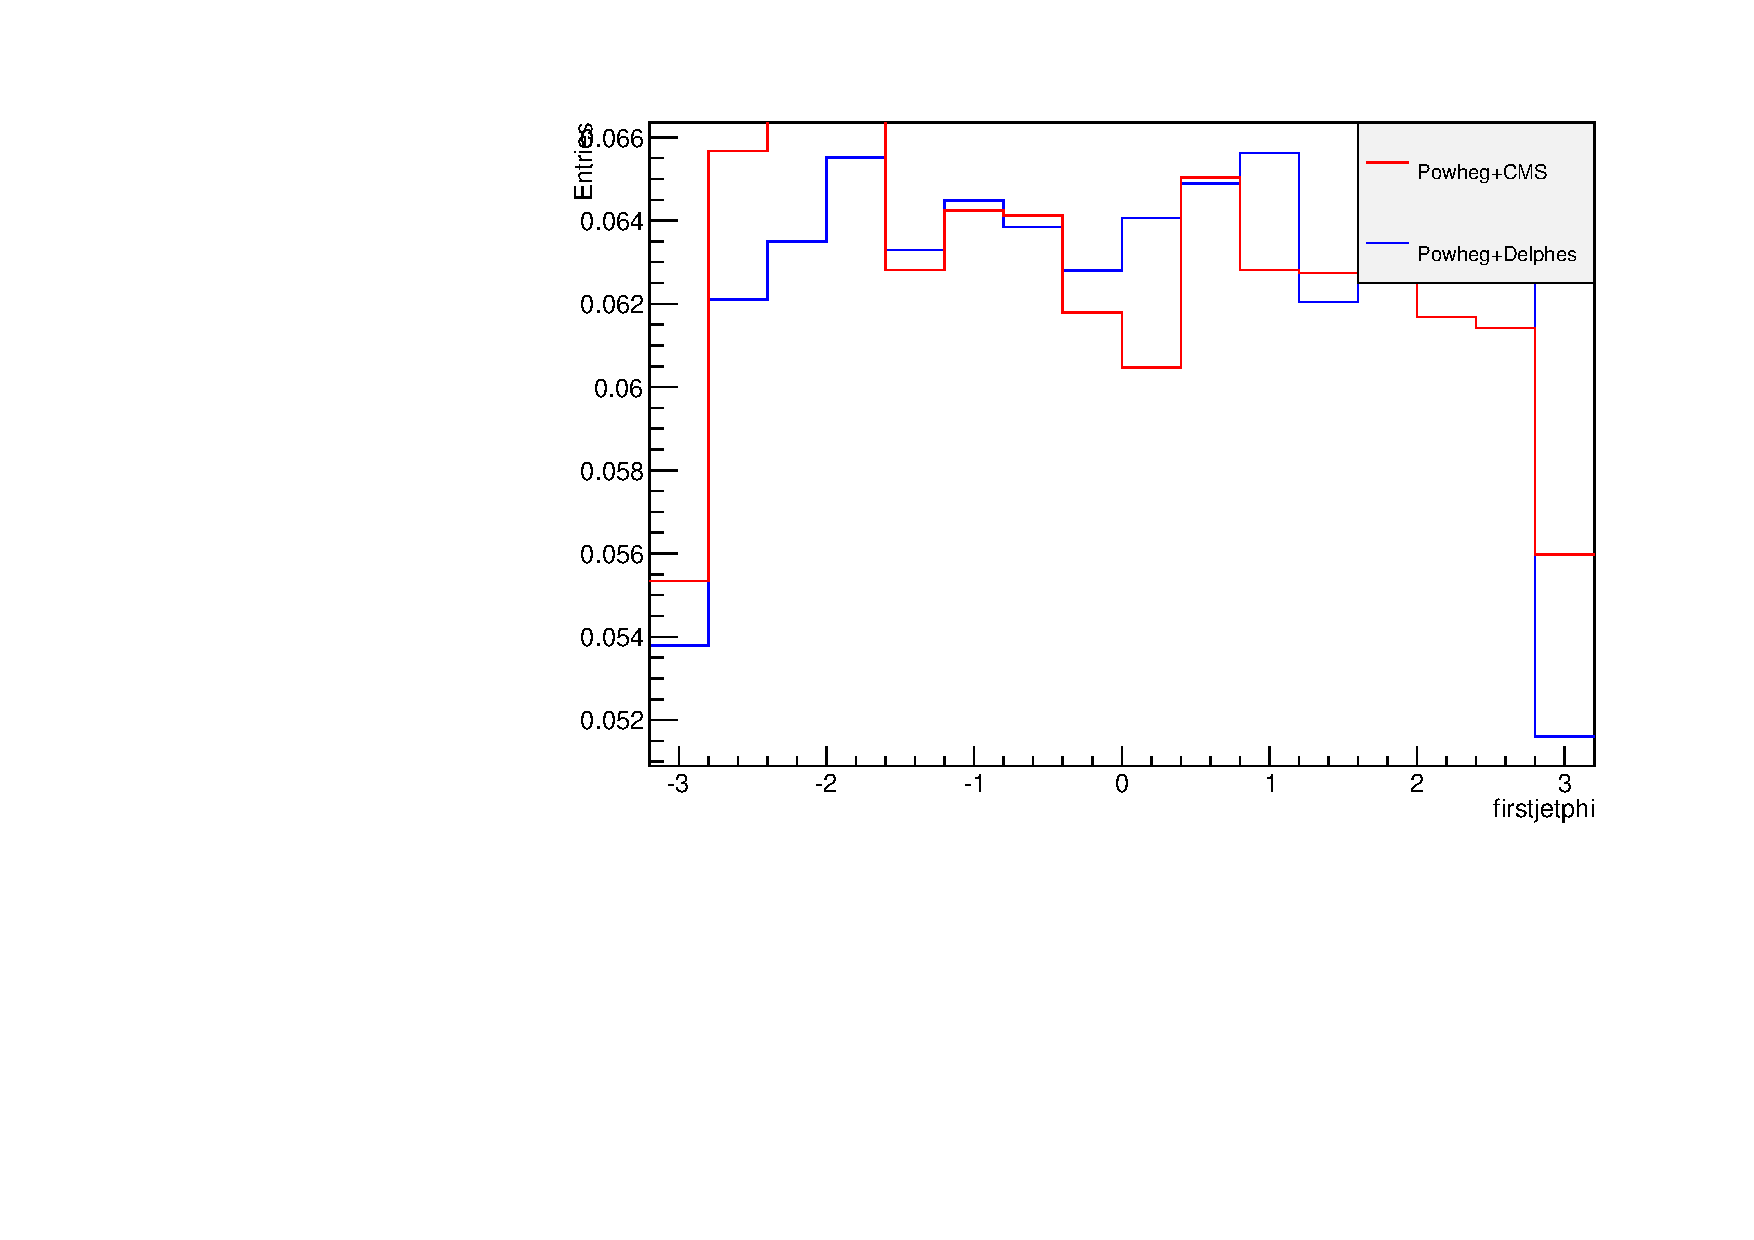
\includegraphics[width=.5\textwidth]{TalkPics/phenoplots201015/firstjetphi_norm.pdf}
  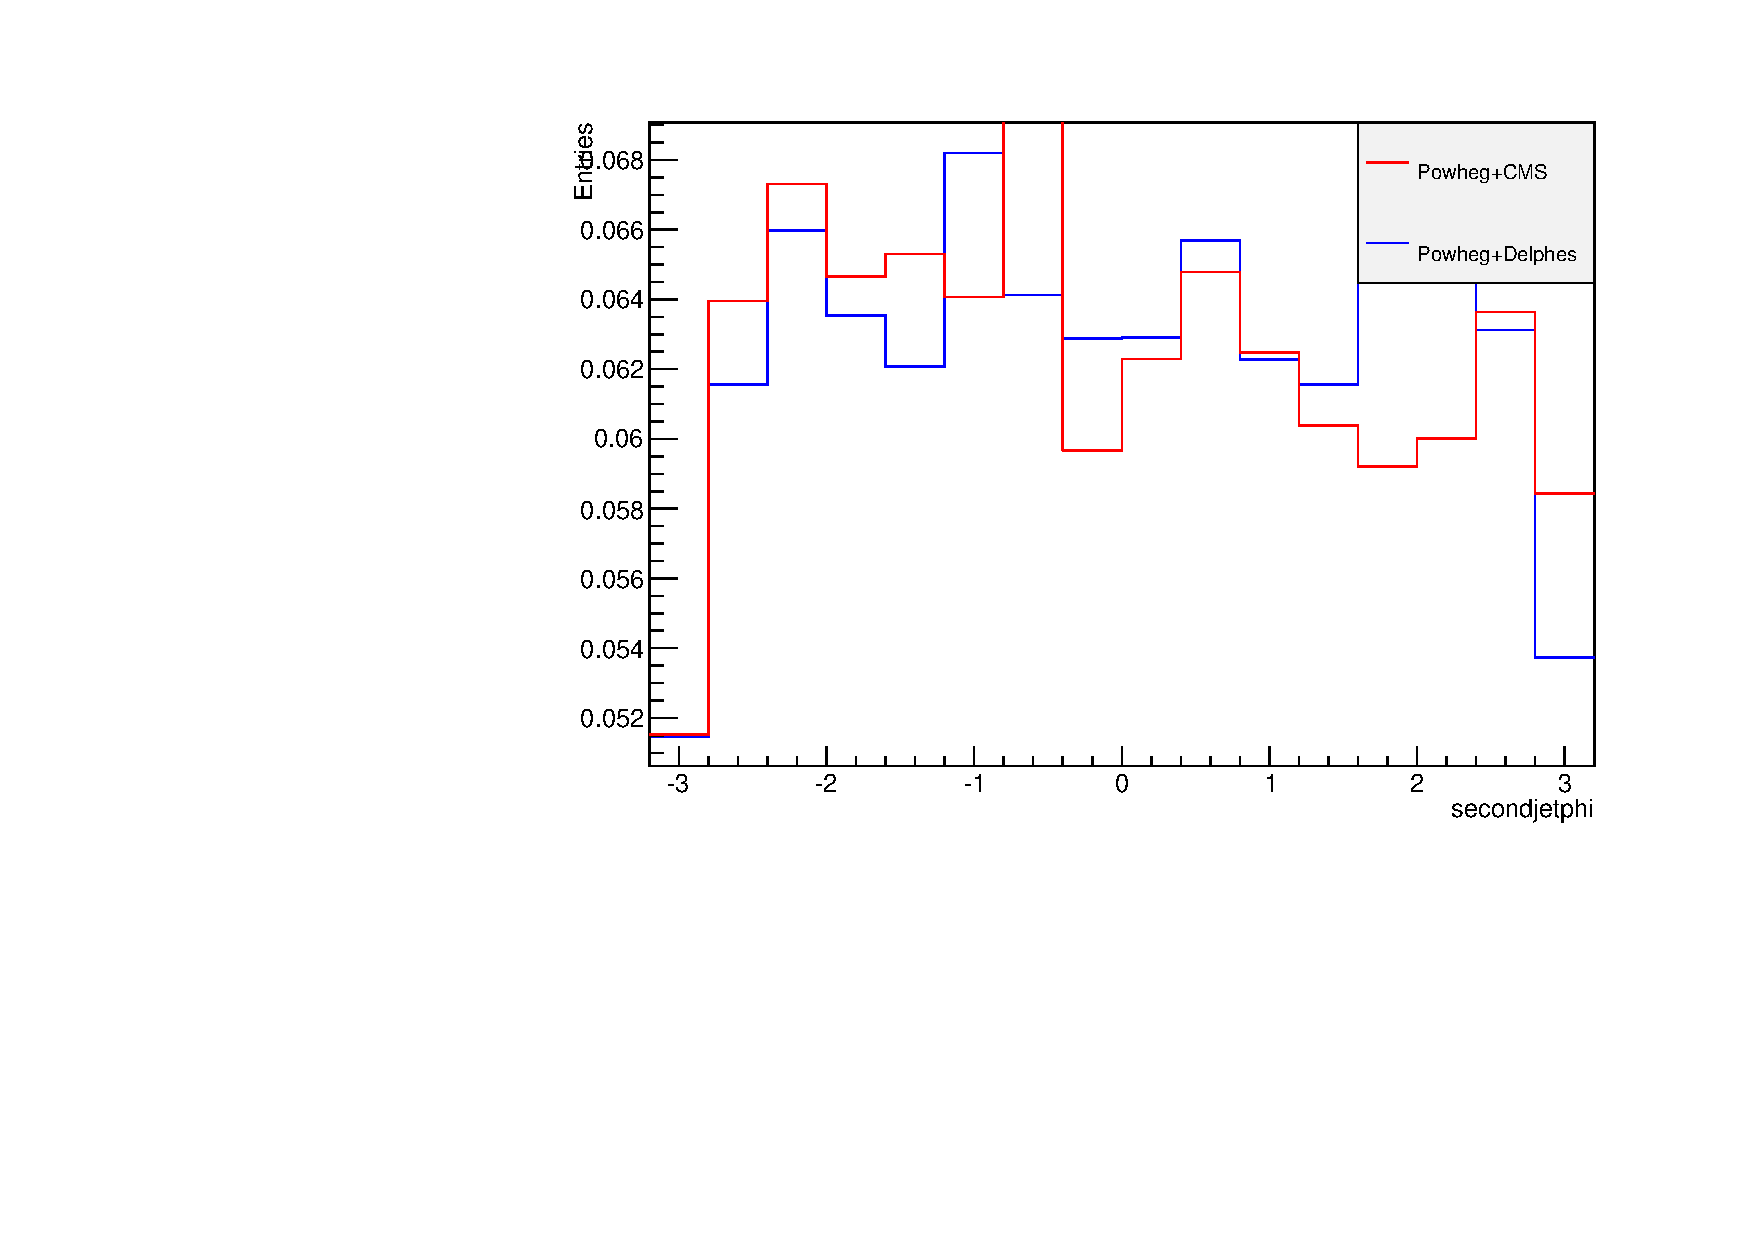
\includegraphics[width=.5\textwidth]{TalkPics/phenoplots201015/secondjetphi_norm.pdf}
    
\end{frame}




\begin{frame}
  \frametitle{Compare Distributions}
  \scriptsize
  \begin{block}{}
    \begin{itemize}
    \item Selection: met significance$>3$, $\Delta\eta_{jj}>3.6$, $j_{1}p_{T}>50$, $j_{2}p_{T}>45$, min$\Delta\phi(j,met)>2.3$, met$>90$
    \item Numbers of jets similar, slightly more additional jets in madgraph
    \end{itemize}
  \end{block}
  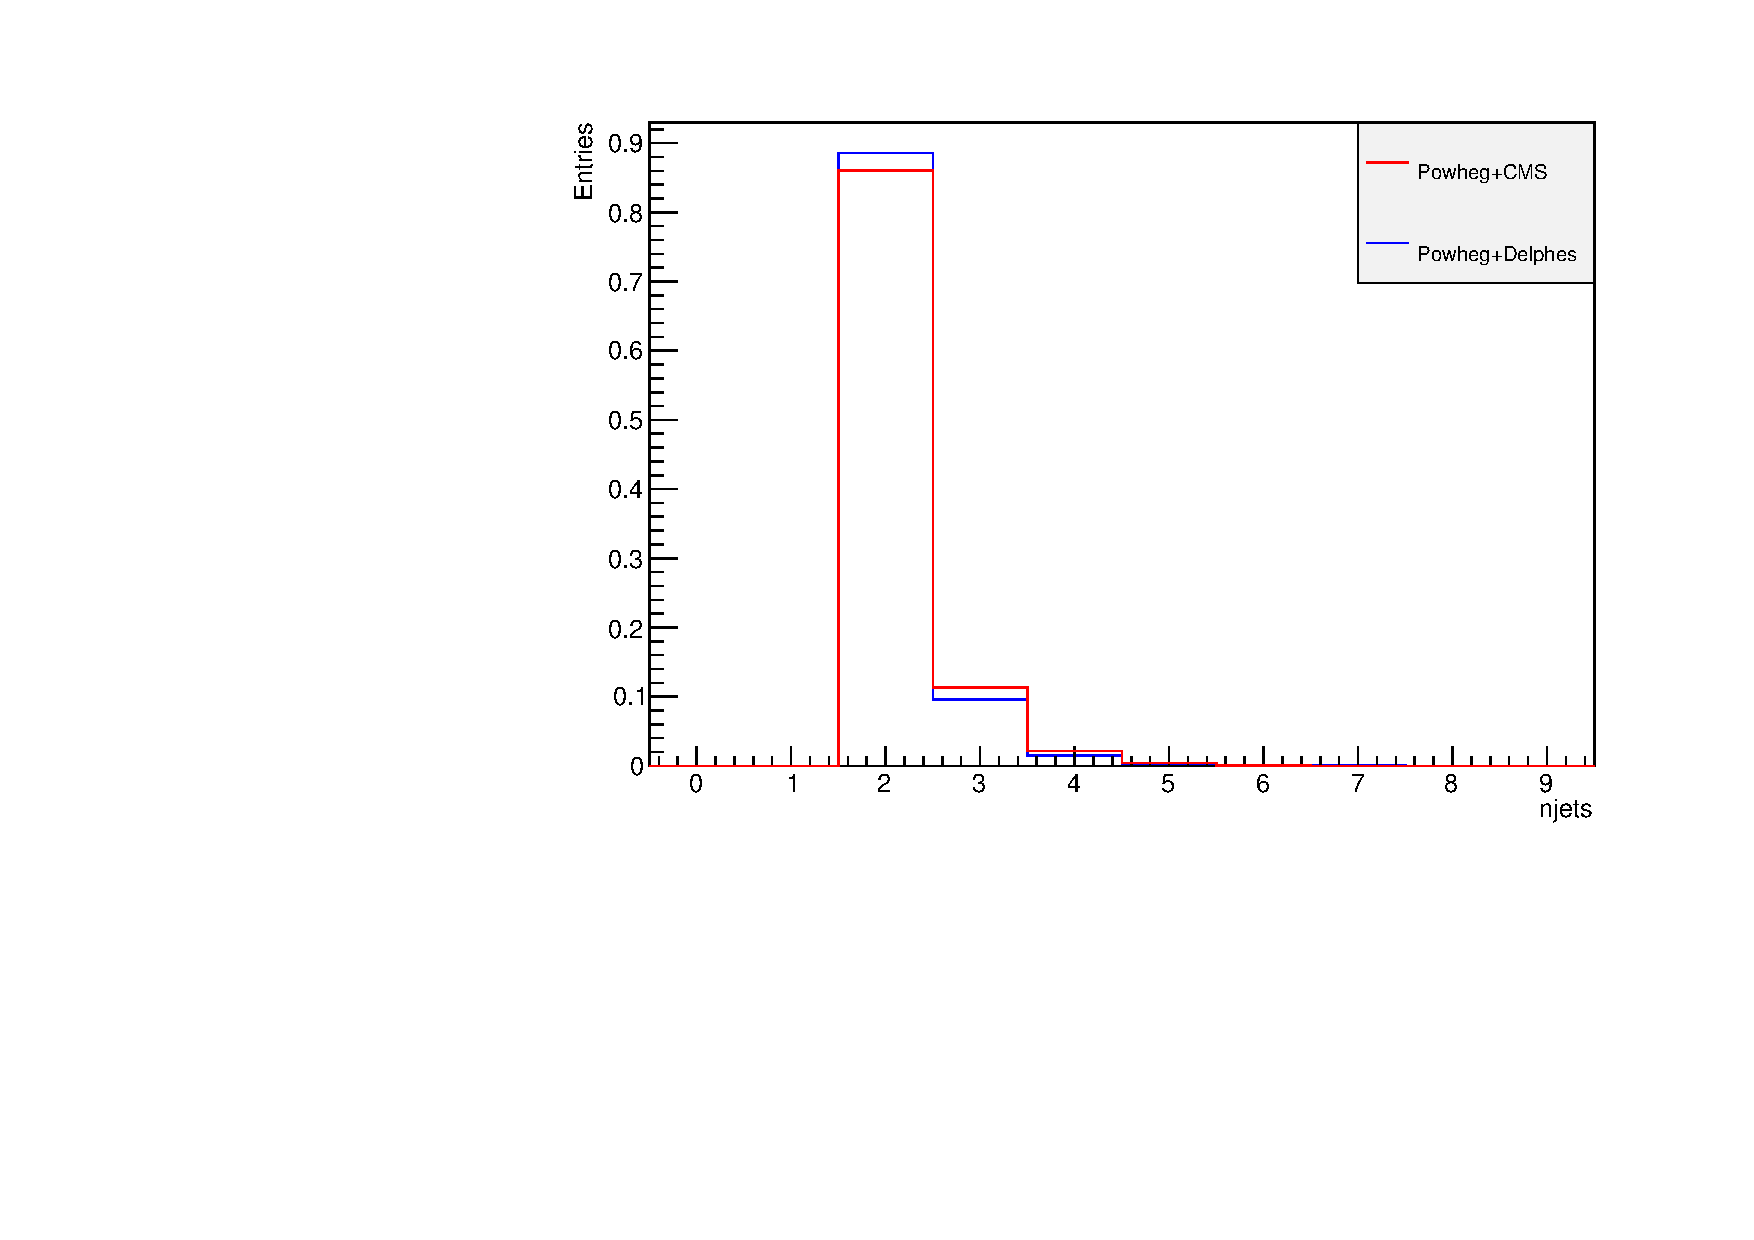
\includegraphics[width=.5\textwidth]{TalkPics/phenoplots201015/njets_norm.pdf}
%  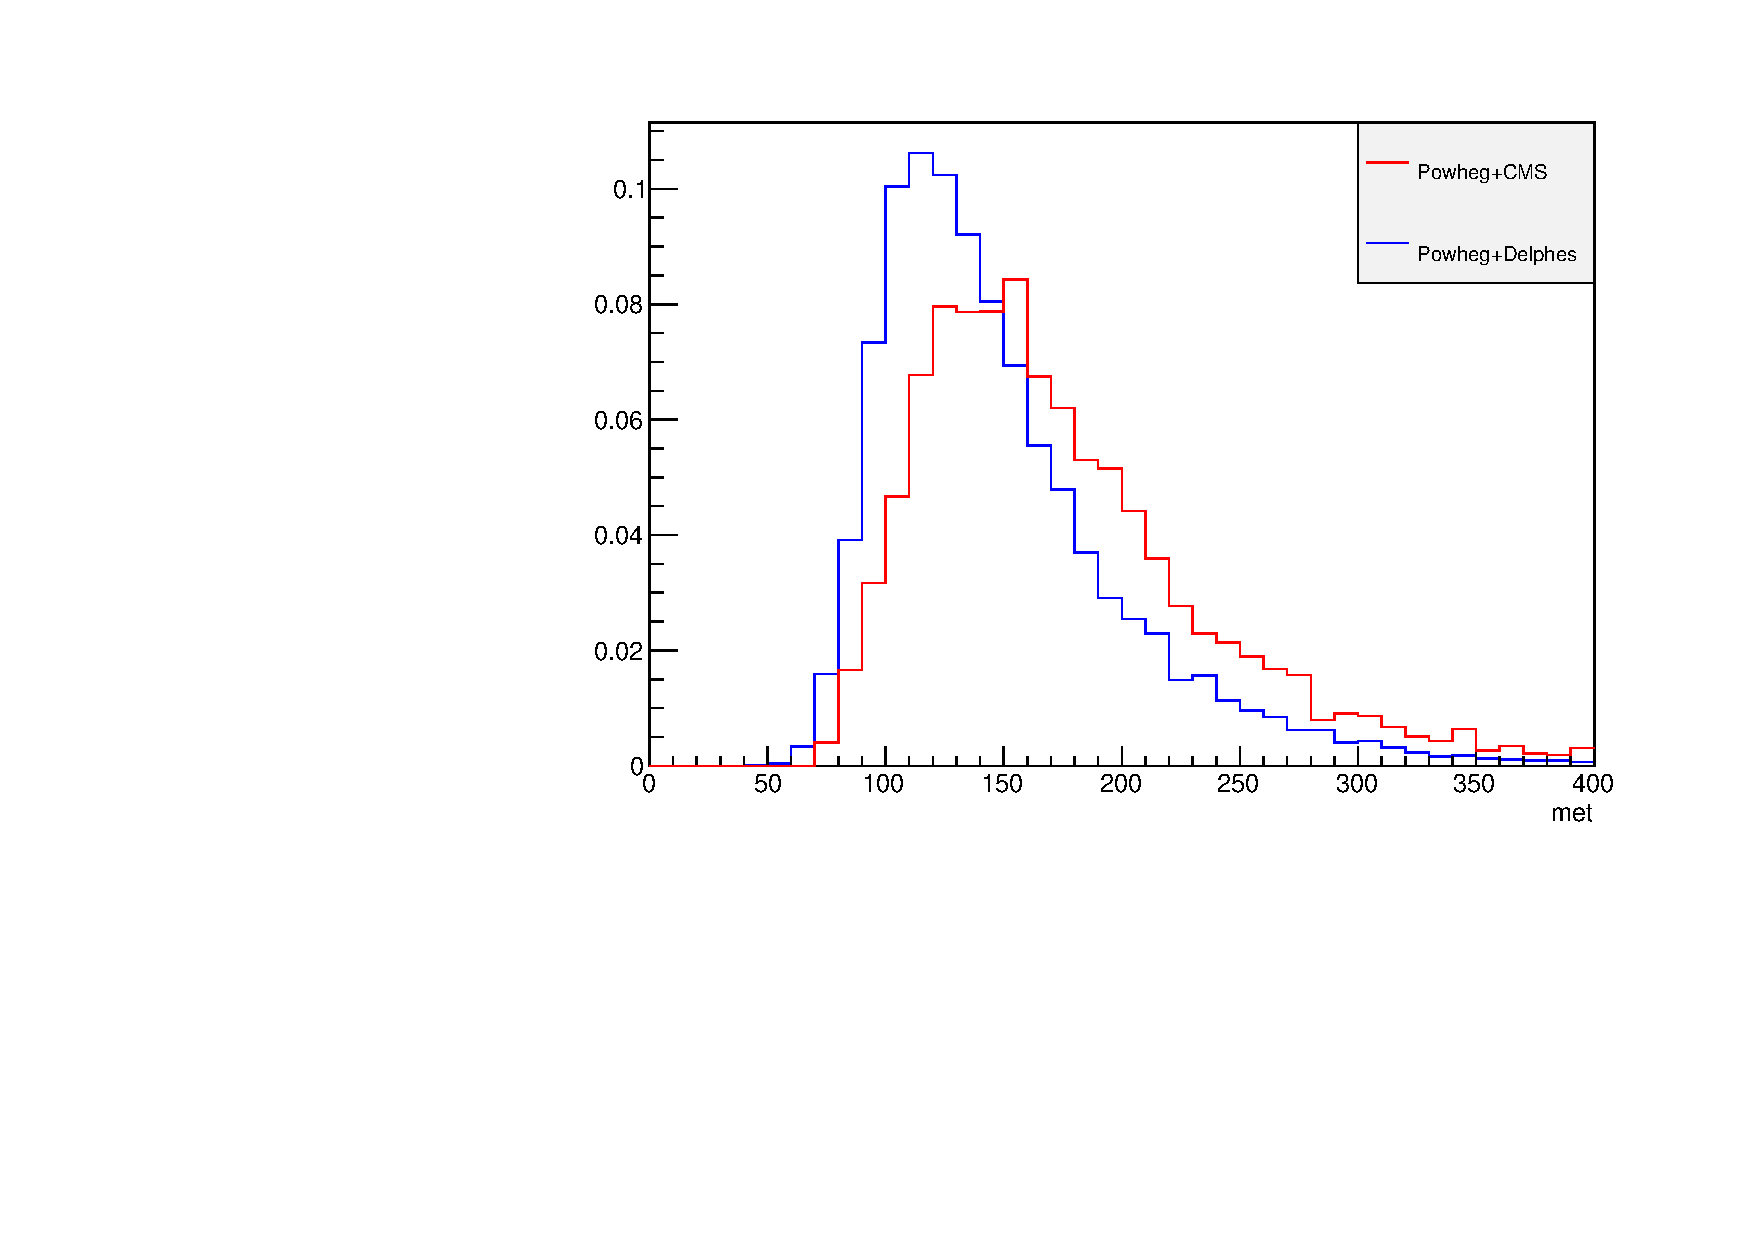
\includegraphics[width=.5\textwidth]{TalkPics/phenoplots201015/met_norm.pdf}
 
    
\end{frame}

\begin{frame}
  \frametitle{Summary}
  \label{lastframe}
  \begin{block}{}
    \scriptsize
    \begin{itemize}
    \item 
    \end{itemize}
  \end{block}
  \centering
  %!!INCLUDE A RUN 2 PLOT
\end{frame}

%UPDATED BACKUP
\begin{frame}
  \frametitle{Backup}
\end{frame}

\end{fmffile}
\end{document}
